% Created 2020-06-25 jeu. 17:24
% Intended LaTeX compiler: pdflatex
\documentclass{ISMA_USD2020}
\usepackage[utf8]{inputenc}
\usepackage[T1]{fontenc}
\usepackage{graphicx}
\usepackage{grffile}
\usepackage{longtable}
\usepackage{wrapfig}
\usepackage{rotating}
\usepackage[normalem]{ulem}
\usepackage{amsmath}
\usepackage{textcomp}
\usepackage{amssymb}
\usepackage{capt-of}
\usepackage{hyperref}
\usepackage[most]{tcolorbox}
\usepackage{bm}
\usepackage{booktabs}
\usepackage{tabularx}
\usepackage{array}
\usepackage{siunitx}
\usepackage{amsmath,amssymb,amsfonts, cases}
\usepackage{algorithmic, graphicx, textcomp}
\usepackage{xcolor, import, hyperref}
\usepackage{subcaption}
\usepackage[USenglish, english]{babel}
\setcounter{footnote}{1}
\usepackage[utf8]{inputenc}
\usepackage[T1]{fontenc}

\usepackage[french, english]{babel} % Last language is main language

\usepackage{lmodern} % Latin Modern Font
\usepackage{gensymb} % Generic symbols for both text and math mode

\usepackage{standalone} % Used to generate standalone Tikz

\usepackage{amsmath}   % Main math Package
\usepackage{mathtools} % Extension package to amsmath
\usepackage{amsthm}    % Typesetting theorems (AMS style)
\usepackage{amsfonts}  % More fonts from the AMS
\usepackage{textcomp}  % provide many text symbols
\usepackage{steinmetz} % For phase symbol

\usepackage{xstring}  % Utils to manipulate strings
\usepackage{etoolbox} % Add basic if/then
\usepackage{esvect}   % Beautyfull vectors
\usepackage{graphicx} % Enhanced support for graphics
\usepackage{grffile}  % Used by matlab2tikz

\usepackage{microtype} % typographic tuning
\usepackage{setspace}  % for line spacing, e.g. \onehalfspacing
\usepackage{tabularx}  % table features
\usepackage{enumitem}  % for simple list modifications
\usepackage{booktabs}  % better table support

\usepackage{stackengine} %

\usepackage[load-configurations=abbreviations]{siunitx} % SI units
\sisetup{
    locale = US,
    detect-all,
    range-phrase=--,
    range-units=single
}

\usepackage{tikz}       % Tikz
\usepackage{tikzscale}  % Used to scale Tikz graphics
\usepackage{adjustbox}  % Used to proper positioning of tikz pictures
\usepackage{circuitikz} % Draw electronic circuits
\usepackage{pgfpages}   % Needed to use notes
\usepackage{pgfplots}   % Used to plot functions

\usetikzlibrary{arrows}                   % Arrow tip library
\usetikzlibrary{arrows.meta}              % Add some arrows
\usetikzlibrary{calc}                     % The library allows advanced Coordinate Calculations
\usetikzlibrary{intersections}            % calculate intersections of paths
\usetikzlibrary{matrix}                   %
\usetikzlibrary{patterns}                 %
\usetikzlibrary{shapes}                   % Defines circle and rectangle
\usetikzlibrary{shapes.geometric}         % Use for the shape diamond and isosceles triangle
\usetikzlibrary{snakes}                   % snake=coil and snake=zigzag using segment amplitude=10pt
\usetikzlibrary{positioning}              % Additional options for placing nodes
\usetikzlibrary{3d}                       % Plot 3D shapes
\usetikzlibrary{spy}                      % Creating a magnified area
\usetikzlibrary{decorations.text}         % Used to make text follows a curve
\usetikzlibrary{decorations.pathmorphing} % deformation of a path
\usetikzlibrary{decorations.markings}     % Used for spring and damper
\usetikzlibrary{babel}                    % A tiny library that make the interaction with the babel package easier
\usetikzlibrary{plotmarks}                % This library defines a number of plot marks
\usetikzlibrary{fit}                      % Used to make rectangle as nodes by specifying two points
\usetikzlibrary{backgrounds}              % Used to put things under others

\usepgfplotslibrary{patchplots}
\usepgfplotslibrary{groupplots}

\pgfplotsset{compat=newest}
\pgfplotsset{plot coordinates/math parser=false}

\newlength{\fheight}
\newlength{\fwidth}

\setlength{\fwidth}{85mm}
\setlength{\fheight}{112mm}

\tikzset{>=Stealth}
% Setup default Linewidth
\tikzset{every path/.style={line width=1pt}}

\usepackage{xcolor}% Color extension

\definecolor{colorblack}{rgb}{0, 0, 0}
\definecolor{colorblue}{rgb}{0, 0.4470, 0.7410}
\definecolor{colorred}{rgb}{0.8500, 0.3250, 0.0980}
\definecolor{coloryellow}{rgb}{0.9290, 0.6940, 0.1250}
\definecolor{colorpurple}{rgb}{0.4940, 0.1840, 0.5560}
\definecolor{colorgreen}{rgb}{0.4660, 0.6740, 0.1880}
\definecolor{colorcyan}{rgb}{0.3010, 0.7450, 0.9330}
\definecolor{colorbordeau}{rgb}{0.6350, 0.0780, 0.1840}

% Main color
\definecolor{maincolor}{RGB}{89, 9, 38}
\definecolor{secondcolor}{RGB}{20, 9, 89}

\tikzset{%
  block/.style n args={2}{%
    draw,
    fill=white,
    minimum width  = #1,
    minimum height = #2,
  },
  block/.default={1.2cm}{1.0cm}
}

\tikzstyle{branch}=[fill,shape=circle,minimum size=4pt,inner sep=0pt]
\tikzstyle{->top}=[-{Stealth[color=black, scale=0.8]}, draw=white, double=black, double distance=1pt, line width=1pt]
\tikzstyle{<-top}=[{stealth[color=black, scale=0.8]}-, draw=white, double=black, double distance=1pt, line width=1pt]

\tikzstyle{handwriten}=[decorate,decoration={random steps,amplitude=0.1pt,segment length=0.8pt}]

\tikzset{%
  DAC/.style={%
    draw,
    signal,
  }
}

\tikzset{%
  ADC/.style={%
    draw,
    signal,
    signal to = west,
  }
}

\tikzset{%
  gain right/.style={%
    draw,
    regular polygon,
    regular polygon sides = 3,
    inner sep = 2pt,
    shape border rotate=-90
  },
  gain left/.style={%
    draw,
    regular polygon,
    regular polygon sides = 3,
    inner sep = 2pt,
    shape border rotate=90
  },
  gain top/.style={%
    draw,
    regular polygon,
    regular polygon sides = 3,
    inner sep = 2pt,
    shape border rotate=0
  },
  gain bottom/.style={%
    draw,
    regular polygon,
    regular polygon sides = 3,
    inner sep = 2pt,
    shape border rotate=180
  },
}

\tikzset{% Add block with Circled operations
  addc/.style n args={5}{%
    draw,
    fill=white,
    circle,
    outer sep = 0pt,
    inner sep = 0pt,
    minimum size = 2em,
    execute at begin node={\LARGE $#1$},
    append after command={\pgfextra{\let\mainnode=\tikzlastnode}
      \ifx#2\empty\else
      node[draw, circle, outer sep=6pt, inner sep=0pt, above left] at (\mainnode.west) {$#2$}%
      \fi
      \ifx#3\empty\else
      node[draw, circle, outer sep=6pt, inner sep=0pt, above right] at (\mainnode.north) {$#3$}%
      \fi
      \ifx#4\empty\else
      node[draw, circle, outer sep=6pt, inner sep=0pt, below right] at (\mainnode.east) {$#4$}%
      \fi
      \ifx#5\empty\else
      node[draw, circle, outer sep=6pt, inner sep=0pt, below left] at (\mainnode.south) {$#5$}%
      \fi
      }
  },
  addc/.default={+}{}{}{}{},
}

\tikzset{% Add Block
  addb/.style n args={5}{%
    draw,
    fill=white,
    circle,
    outer sep = 0pt,
    inner sep = 0pt,
    minimum size = 2em,
    execute at begin node={\LARGE $#1$},
    append after command={\pgfextra{\let\mainnode=\tikzlastnode}
      \ifx#2\empty\else
      node[outer sep=2pt, inner sep=0pt, above left] at (\mainnode.west) {$#2$}%
      \fi
      \ifx#3\empty\else
      node[outer sep=2pt, inner sep=0pt, above right] at (\mainnode.north) {$#3$}%
      \fi
      \ifx#4\empty\else
      node[outer sep=2pt, inner sep=0pt, below right] at (\mainnode.east) {$#4$}%
      \fi
      \ifx#5\empty\else
      node[outer sep=2pt, inner sep=0pt, below left] at (\mainnode.south) {$#5$}%
      \fi
      }
  },
  addb/.default={+}{}{}{}{},
}

\pgfplotsset{grid style={black}}
\pgfplotsset{major grid style={black!30!white}}
\pgfplotsset{minor grid style={black!10!white}}
\pgfplotsset{xmajorgrids}
\pgfplotsset{ymajorgrids}

\pgfplotsset{separate axis lines=false} % draw axis as rectangle and not as 4 lines
\pgfplotsset{every outer x axis line/.append style={black}}
\pgfplotsset{every outer y axis line/.append style={black}}
\pgfplotsset{axis background/.style={fill=white}}
\pgfplotsset{axis x line*=bottom} % solid line on the bottom with thin on the top
\pgfplotsset{axis y line*=left} % solid line on the left with thin on the right

\pgfplotsset{every y tick label/.append style={font=\color{black}}}
\pgfplotsset{every y tick/.append style={black}}
\pgfplotsset{every x tick label/.append style={font=\color{black}}}
\pgfplotsset{every x tick/.append style={black}}

\pgfplotsset{scale only axis=true}

\pgfplotsset{ylabel absolute}

% https://tex.stackexchange.com/questions/54794/using-a-pgfplots-style-legend-in-a-plain-old-tikzpicture#54834

% argument #1: any options
\newenvironment{customlegend}[1][]{%
  \begingroup
  % inits/clears the lists (which might be populated from previous
  % axes):
  \csname pgfplots@init@cleared@structures\endcsname
  \pgfplotsset{#1}%
}{%
  % draws the legend:
  \csname pgfplots@createlegend\endcsname
  \endgroup
}%

% makes \addlegendimage available (typically only available within an
% axis environment):
\def\addlegendimage{\csname pgfplots@addlegendimage\endcsname}

% definition to insert numbers
% \pgfkeys{/pgfplots/number in legend/.style={%
%     /pgfplots/legend image code/.code={%
%       \node at (0.125,-0.0225){#1}; % <= changed x value
%     },%
%   },
% }
\pgfplotsset{
  every legend to name picture/.style={west}
}

\tikzstyle{upperbound}=[line cap=round, postaction={decorate,draw,decoration={border, segment length=0.2cm, amplitude=0.3cm, angle=60}}]
\tikzstyle{lowerbound}=[line cap=round, postaction={decorate,draw,decoration={border, segment length=0.2cm, amplitude=0.3cm, angle=-60}}]

\pgfplotsset{
  /pgfplots/upperbound/.style 1 args={
    legend image code/.code={
      \draw[##1, upperbound]
        plot coordinates {
        (0cm,0cm)
        (0.6cm,0cm)
      }
    }
  }
}

\tikzset{%
  pole/.style{%
    color=red,
    cross out,
    draw,
    inner sep=0pt,
    outer sep=0pt,
    minimum size=#1pt
  },
  pole/.default={4}
}

\tikzset{%
  zero/.style{%
    color=red,
    circle,
    draw,
    inner sep=0pt,
    outer sep=0pt,
    minimum size=#1pt
  },
  zero/.default={4}
}

\tikzset{%
  spring/.style={%
    thick,
    decoration={
      zigzag,
      pre length  = #1cm,
      post length = #1cm,
      segment length = 6
    },
    decorate
  },
  spring/.default={0.2}
}

\tikzset{%
  coil/.style n args={2}{%
    thick,
    decoration={
      coil,
      pre length  = #1cm,
      post length = #2cm,
      segment length = 4
    },
    decorate
  },
  coil/.default={0.3}{0.3}
}

\tikzset{%
  damper/.style n args={2}{%
    thick,
    decoration={markings, mark connection node=dmp, mark=at position 0.5 with {
        \node (dmp) [thick,
                     inner sep = 0pt,
                     transform shape,
                     rotate  =-90,
                     minimum width  = #1pt,
                     minimum height = #2pt,
                     draw=none] {};
        \draw [thick] ($(dmp.north east)+(0.6*#2pt,0)$) -- (dmp.south east) -- (dmp.south west) -- ($(dmp.north west)+(0.6*#2pt,0)$);
        \draw [thick] ($(dmp.north)+(0,-0.3*#1pt)$) -- ($(dmp.north)+(0,0.3*#1pt)$);
      }
    },
    decorate
  },
  damper/.default={12}{3}
}

\tikzset{%
  actuator/.style n args={2}{%
    thick,
    draw=none,
    decoration={
      markings,
      mark connection node=my node,
      mark=at position .5 with {
        \node [draw, inner sep=0pt, minimum width=#1cm, minimum height=#2cm,
        transform shape, fill=white] (my node) {};
      },
      mark=at position .0 with {
        \draw[<-] (0, 0) -- (my node);
      },
      mark=at position 1.0 with {
        \draw[<-] (0, 0) -- (my node);
      }
    },
    decorate
  },
  actuator/.default={0.5}{0.2}
}

\tikzset{%
  ground/.style n args={2}{%
    fill,
    pattern = north east lines,
    draw = none,
    anchor = north,
    minimum width  = #1cm,
    minimum height = #2cm,
    append after command={
      (\tikzlastnode.north west) edge (\tikzlastnode.north east)
    }
  },
  ground/.default={2.5}{0.3}
}

\tikzset{%
  forcesensor/.style n args={2}{%
    rectangle,
    outer sep=0pt,
    inner sep=0pt,
    draw=black,
    fill=white!60!black,
    anchor=south,
    minimum width =#1cm,
    minimum height=#2cm,
    append after command={
      [every edge/.append style={
        thick,
        black,
      }]
      (\tikzlastnode.north west) edge (\tikzlastnode.south east)
      (\tikzlastnode.north east) edge (\tikzlastnode.south west)
    }
  },
  forcesensor/.default={2.0}{0.5}
}

\tikzset{%
  inertialsensor/.style={%
    rectangle,
    outer sep=0pt,
    inner sep=0pt,
    draw=black,
    fill=white!60!black,
    anchor=south east,
    minimum size=#1cm,
    append after command={
      [every edge/.append style={
        thick,
        black,
      }]
      (\tikzlastnode.north west) edge (\tikzlastnode.south east)
      (\tikzlastnode.north east) edge (\tikzlastnode.south west)
    }
  },
  inertialsensor/.default={0.3}
}

\newcommand{\AxisRotator}[1][rotate=0]{%
  \tikz [x=0.1cm,y=0.30cm,-stealth,#1] \draw (0,0) arc (-150:150:1 and 1);%
}

\tikzstyle{cross}=[path picture={
  \draw[black]
  (path picture bounding box.south east) -- (path picture bounding box.north west) (path picture bounding box.south west) -- (path picture bounding box.north east);
}]

\tikzset{%
  piezo/.style n args={3}{%
    draw,
    rectangle,
    minimum width  = #1cm,
    minimum height = #2cm,
    fill=blue!10!white,
    anchor=center,
    append after command={
      [every edge/.append style={
        thick,
        black,
      }]
      \foreach \i in {1,...,#3}{
        (${\i/(1+#3)}*(\tikzlastnode.north west)+{(1+#3-\i)/(1+#3)}*(\tikzlastnode.south west)+0.1*(#1,0)$) edge (${\i/(1+#3)}*(\tikzlastnode.north east)+{(1+#3-\i)/(1+#3)}*(\tikzlastnode.south east)-0.1*(#1,0)$)
      }
    }
  },
  piezo/.default={2}{4}{10}
}

\def\voicecoil#1#2#3{
  % ======================
  % Parameters
  % ======================
  \def\voicecoilw{#1} % Total Width
  \def\voicecoilh{#2} % Total Height

  \def\magnetw{\voicecoilw} % Width of the magnet
  \def\magneth{\voicecoilh/1.4} % Height of the magnet

  \def\magnetwb{0.15*\magnetw} % Width of the borders of the magnet
  \def\magnetmw{0.15*\magnetw} % Width of the middle part of the magnet
  \def\magnetwg{0.5*\magnetw} % Width of the gap of the magnet

  \def\magnethl{\magnetwb} % Height of the low part of the magnet
  \def\magnetmh{0.15*\magneth} % Height of the middle part of the magnet
  \def\magnethg{0.2*\magneth} % Height of the gap of the magnet
  % ======================

  \begin{scope}[shift={(0.5*\voicecoilw, 0.5*\voicecoilh)}, rotate=#3, shift={(0, -0.5*\voicecoilh)}]
    % ======================
    % Magnet
    % ======================
    \draw[fill=white] (0, 0) -| ++(0.5*\magnetw, \magneth) -| ++(-0.5*\magnetw+0.5*\magnetwg, -\magnethg) -| (0.5*\magnetw-\magnetwb, \magnethl) -| (-0.5*\magnetw+\magnetwb, \magneth-\magnethg) -| (-0.5*\magnetwg, \magneth) -| (-0.5*\magnetw, 0) -- (cycle);
    \begin{scope}[shift={(0, \magnethl)}]
      \draw[fill=red]  (-0.5*\magnetmw, 0) rectangle (0.5*\magnetmw, \magnetmh);
      \draw[fill=blue] (-0.5*\magnetmw, \magnetmh) rectangle (0.5*\magnetmw, 2*\magnetmh);
      % Top conductive Magnet
      \draw[fill=white] (-0.5*\magnetmw, 2*\magnetmh) -| (0.5*\magnetmw, -\magnethl+\magneth-\magnethg) -| ++(0.1, \magnethg) -| ++(-0.2-\magnetmw, -\magnethg) -| (-0.5*\magnetmw, \magnetmh);
    \end{scope}
    % ======================

    % ======================
    % Coil
    % ======================
    \pgfmathsetmacro{\coilwidth}{0.5*0.5*\magnetmw+0.5*0.1+0.25*\magnetwg}%
    \draw[] ( \coilwidth, 0.5*\magneth) -- ++(0, 0.7*\magneth);
    \draw[] (-\coilwidth, 0.5*\magneth) -- ++(0, 0.7*\magneth);
    % Point on the coil
    \foreach \x in {0,1,...,9}
    {
      \node[circle,inner sep=0.6pt,fill] at ( \coilwidth, \x*0.7*\magneth/10+0.5*\magneth);
      \node[circle,inner sep=0.6pt,fill] at (-\coilwidth, \x*0.7*\magneth/10+0.5*\magneth);
    }
    \draw[fill=white] (-0.5*\magnetw, 1.2*\magneth) rectangle ++(\magnetw, \magnethg);
    % ======================

    % ======================
    % Coordinates
    % ======================
    % Force
    \coordinate[] (vc_force) at (0, \magneth-0.5*\magnethg);
    % Coil
    \coordinate[] (vc_coil) at (0, \voicecoilh);
    % Magnet
    \coordinate[] (vc_magnet) at (0, 0);
    % Coil Wires
    \coordinate[] (vc_wire_one) at ( \coilwidth, 1.2*\magneth);
    \coordinate[] (vc_wire_two) at (-\coilwidth, 1.2*\magneth);
    % ======================
  \end{scope}
}

\tikzset{%
  ->-/.style={
    decoration={
      markings,
      mark = at position #1 with {\arrow{>}
      }
    },
    postaction={decorate}
  }
}
\tikzset{%
  -<-/.style={
    decoration={
      markings,
      mark = at position #1 with {\arrow{<}
      }
    },
    postaction={decorate}
  }
}

\tikzset{%
  labelc/.style= {%
    draw,
    fill=white,
    shape=circle,
    inner sep=2pt,
    outer sep=6pt,
  }
}

\author[1,3] {T. Dehaeze}
\author[1,2] {C. Collette}
\affil[1] {Precision Mechatronics Laboratory\NewLineAffil University of Liege, Belgium \NewAffil}
\affil[2] {BEAMS Department\NewLineAffil Free University of Brussels, Belgium \NewAffil}
\affil[3] {European Synchrotron Radiation Facility \NewLineAffil Grenoble, France e-mail: \textbf{thomas.dehaeze@esrf.fr}}
\bibliographystyle{IEEEtran}
\usepackage{tikz}
\usetikzlibrary{shapes.misc}
\date{}
\title{Decentralized Active Damping of Rotating Positioning Platforms}
\hypersetup{
 pdfauthor={},
 pdftitle={Decentralized Active Damping of Rotating Positioning Platforms},
 pdfkeywords={},
 pdfsubject={},
 pdfcreator={Emacs 27.0.91 (Org mode 9.4)}, 
 pdflang={English}}
\begin{document}

\maketitle

\abstract{
    Abstract text to be done
}

\section{Introduction}
\label{sec:org7ff5c70}
\label{sec:introduction}
Controller Poles are shown by black crosses (
\begin{tikzpicture} \node[cross out, draw=black, minimum size=1ex, line width=2pt, inner sep=0pt, outer sep=0pt] at (0, 0){}; \end{tikzpicture}
).
Due to gyroscopic effects, the guaranteed robustness properties of Integral Force Feedback do not hold.
Either the control architecture can be slightly modfied or mechanical changes in the system can be performed.
This paper has been published
The Matlab code that was use to obtain the results are available in \cite{dehaeze20_activ_dampin_rotat_posit_platf}.

\section{Dynamics of Rotating Positioning Platforms}
\label{sec:org029ca48}
\subsection{Studied Rotating Positioning Platform}
\label{sec:org7eec6c5}
Consider the rotating X-Y stage of Figure \ref{fig:system}.

\begin{itemize}
\item \(k\): Actuator's Stiffness [N/m]
\item \(m\): Payload's mass [kg]
\item \(\Omega = \dot{\theta}\): rotation speed [rad/s]
\item \(F_u\), \(F_v\)
\item \(d_u\), \(d_v\)
\end{itemize}

\begin{figure}[htbp]
\centering
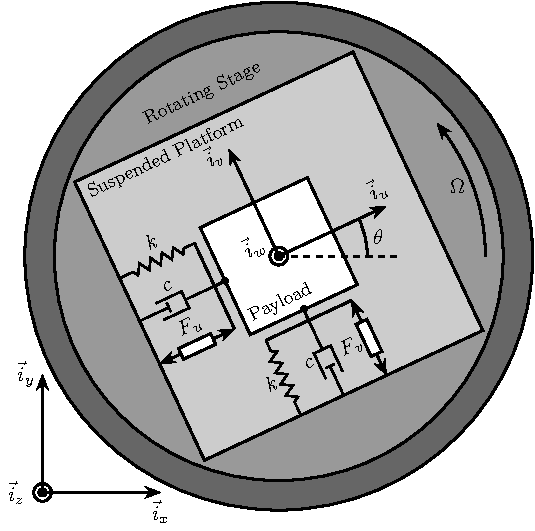
\includegraphics[scale=1]{figs/system.pdf}
\caption{\label{fig:system}Schematic of the studied System}
\end{figure}

\subsection{Equations of Motion}
\label{sec:orgca181a2}
The system has two degrees of freedom and is thus fully described by the generalized coordinates \([q_1\ q_2] = [d_u\ d_v]\) (describing the position of the mass in the rotating frame).

Let's express the kinetic energy \(T\), the potential energy \(V\) of the mass \(m\) (neglecting the rotational energy) as well as the deceptive function \(R\):
\begin{subequations}
\label{eq:energy_functions_lagrange}
  \begin{align}
    T & = \frac{1}{2} m \left( \left( \dot{d}_u - \Omega d_v \right)^2 + \left( \dot{d}_v + \Omega d_u \right)^2 \right) \\
    V & = \frac{1}{2} k \left( {d_u}^2 + {d_v}^2 \right) \\
    R & = \frac{1}{2} c \left( \dot{d}_u{}^2 + \dot{d}_v{}^2 \right)
  \end{align}
\end{subequations}

The equations of motion are derived from the Lagrangian equation:
\begin{equation}
\label{eq:lagrangian_equations}
  \frac{d}{dt} \left( \frac{\partial L}{\partial \dot{q}_i} \right) + \frac{\partial D}{\partial \dot{q}_i} - \frac{\partial L}{\partial q_i} = Q_i
\end{equation}
with \(L = T - V\) is the Lagrangian and \(Q_i\) is the generalized force associated with the generalized variable \(q_i\) (\(Q_1 = F_u\) and \(Q_2 = F_v\)).

\begin{subequations}
\label{eq:eom_coupled}
  \begin{align}
    m \ddot{d}_u + c \dot{d}_u + ( k - m \Omega ) d_u &= F_u + 2 m \Omega \dot{d}_v \\
    m \ddot{d}_v + c \dot{d}_v + ( k \underbrace{-\,m \Omega}_{\text{Centrif.}} ) d_v &= F_v \underbrace{-\,2 m \Omega \dot{d}_u}_{\text{Coriolis}}
  \end{align}
\end{subequations}

The Gyroscopic effects can be seen from the two following terms:
\begin{itemize}
\item Coriolis Forces: coupling
\item Centrifugal forces: negative stiffness
\end{itemize}

\subsection{Transfer Functions in the Laplace domain}
\label{sec:orge7e184a}

Using the Laplace transformation on the equations of motion \eqref{eq:eom_coupled}, the transfer functions from \([F_u,\ F_v]\) to \([d_u,\ d_v]\) are obtained:
\begin{subequations}
\label{eq:oem_laplace_domain}
  \begin{align}
    d_u &= \frac{ms^2 + cs + k - m \Omega^2}{\left( m s^2 + cs + k - m \Omega^2 \right)^2 + \left( 2 m \Omega s \right)^2} F_u +  \frac{2 m \Omega s}{\left( m s^2 + cs + k - m \Omega^2 \right)^2 + \left( 2 m \Omega s \right)^2} F_v \\
    d_v &= \frac{-2 m \Omega s}{\left( m s^2 + cs + k - m \Omega^2 \right)^2 + \left( 2 m \Omega s \right)^2} F_u +  \frac{ms^2 + cs + k - m \Omega^2}{\left( m s^2 + cs + k - m \Omega^2 \right)^2 + \left( 2 m \Omega s \right)^2} F_v
  \end{align}
\end{subequations}


Without rotation \(\Omega = 0\) and the system corresponds to two uncoupled one degree of freedom mass-spring-damper systems:
\begin{subequations}
\label{eq:oem_no_rotation}
  \begin{align}
    d_u &= \frac{1}{m s^2 + cs + k} F_u \\
    d_v &= \frac{1}{m s^2 + cs + k} F_v
  \end{align}
\end{subequations}

\subsection{Change of Variables / Parameters for the study}
\label{sec:org3cdb1ab}

In order this study is more independent on the system parameters, the following change of variable is performed:
\begin{itemize}
\item \(\omega_0 = \sqrt{\frac{k}{m}}\): Natural frequency of the mass-spring system in \(\si{\radian/\s}\)
\item \(\xi = \frac{c}{2 \sqrt{k m}}\): Damping ratio
\end{itemize}

\begin{equation}
\label{eq:tf_d}
  \begin{bmatrix} d_u \\ d_v \end{bmatrix} = \bm{G}_d \begin{bmatrix} F_u \\ F_v \end{bmatrix}
\end{equation}
Where \(\bm{G}_d\) is a \(2 \times 2\) transfer function matrix.

\begin{equation}
\bm{G}_d = \frac{1}{k} \frac{1}{G_{dp}}
\begin{bmatrix}
   G_{dz} & G_{dc} \\
  -G_{dc} & G_{dz}
\end{bmatrix}
\end{equation}
With:
\begin{subequations}
  \begin{align}
    G_{dp} &= \left( \frac{s^2}{{\omega_0}^2} + 2 \xi \frac{s}{\omega_0} + 1 - \frac{{\Omega}^2}{{\omega_0}^2} \right)^2 + \left( 2 \frac{\Omega}{\omega_0} \frac{s}{\omega_0} \right)^2 \\
    G_{dz} &= \frac{s^2}{{\omega_0}^2} + 2 \xi \frac{s}{\omega_0} + 1 - \frac{{\Omega}^2}{{\omega_0}^2} \\
    G_{dc} &= 2 \frac{\Omega}{\omega_0} \frac{s}{\omega_0}
  \end{align}
\end{subequations}

\(G_{dp}\) describes to poles of the system, \(G_{dz}\) the zeros of the diagonal terms and \(G_{dc}\) the coupling.

\begin{itemize}
\item \(k = \SI{1}{N/m}\), \(m = \SI{1}{kg}\), \(c = \SI{0.05}{\newton\per\meter\second}\)
\item \(\omega_0 = \SI{1}{\radian\per\second}\), \(\xi = 0.025\)
\end{itemize}

\subsection{System Dynamics and Campbell Diagram}
\label{sec:org42dee20}
The bode plot of \(\bm{G}_d\) is shown in Figure \ref{fig:plant_compare_rotating_speed}.

\begin{figure}[htbp]
\begin{subfigure}[c]{0.45\linewidth}
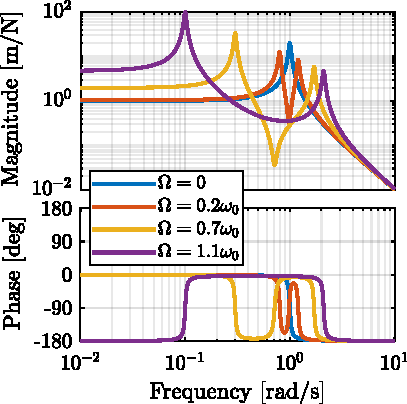
\includegraphics[width=\linewidth]{figs/plant_compare_rotating_speed_direct.pdf}
\caption{\label{fig:plant_compare_rotating_speed_direct} Direct Terms \(d_u/F_u\), \(d_v/F_v\)}
\end{subfigure}
\begin{subfigure}[c]{0.45\linewidth}
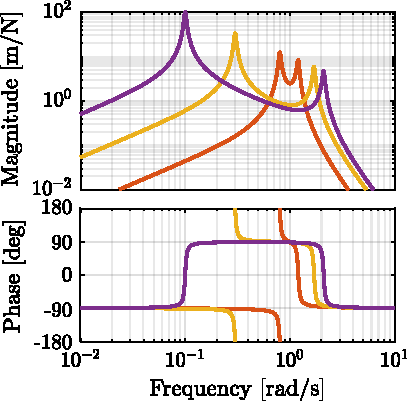
\includegraphics[width=\linewidth]{figs/plant_compare_rotating_speed_coupling.pdf}
\caption{\label{fig:plant_compare_rotating_speed_coupling} Coupling Terms \(d_v/F_u\), \(d_u/F_v\)}
\end{subfigure}
\caption{\label{fig:plant_compare_rotating_speed}Bode Plots for \(\bm{G}_d\)}
\centering
\end{figure}


The poles are the roots of \(G_{dp}\).
Two pairs of complex conjugate poles (supposing small damping \(\xi \approx 0\)):
\begin{subequations}
  \begin{align}
    p_1 &= \pm j (\omega_0 - \Omega) \\
    p_2 &= \pm j (\omega_0 + \Omega)
  \end{align}
\end{subequations}

When the rotation speed in non-null, the resonance frequency is split into two pairs of complex conjugate poles.
As the rotation speed increases, one of the two resonant frequency goes to lower frequencies as the other one goes to higher frequencies.

When the rotational speed \(\Omega\) reaches \(\omega_0\), the real part of one pair of complex conjugate becomes position meaning is system is unstable.

The stiffness of the X-Y stage is too small to hold to rotating payload hence the instability.

Stiff positioning platforms should be used if high rotational speeds or heavy payloads are used.

\begin{figure}[htbp]
\begin{subfigure}[c]{0.4\linewidth}
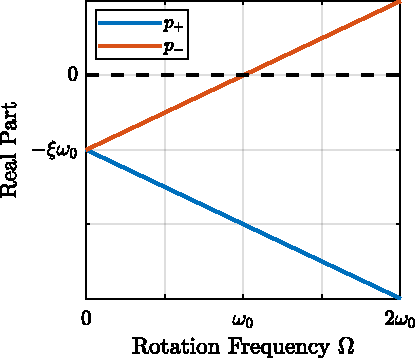
\includegraphics[width=\linewidth]{figs/campbell_diagram_real.pdf}
\caption{\label{fig:campbell_diagram_real} Real Part}
\end{subfigure}
\begin{subfigure}[c]{0.4\linewidth}
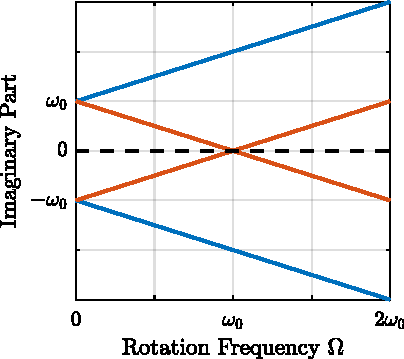
\includegraphics[width=\linewidth]{figs/campbell_diagram_imag.pdf}
\caption{\label{fig:campbell_diagram_imag} Imaginary Part}
\end{subfigure}
\caption{\label{fig:campbell_diagram}Campbell Diagram : Evolution of the poles as a function of the rotational speed \(\Omega\)}
\centering
\end{figure}

\section{Decentralized Integral Force Feedback}
\label{sec:orgda38ad7}
\subsection{System Schematic and Control Architecture}
\label{sec:orgf08eb9d}

Force Sensors are added in series with the actuators as shown in Figure \ref{fig:system_iff}.

\begin{figure}[htbp]
\centering
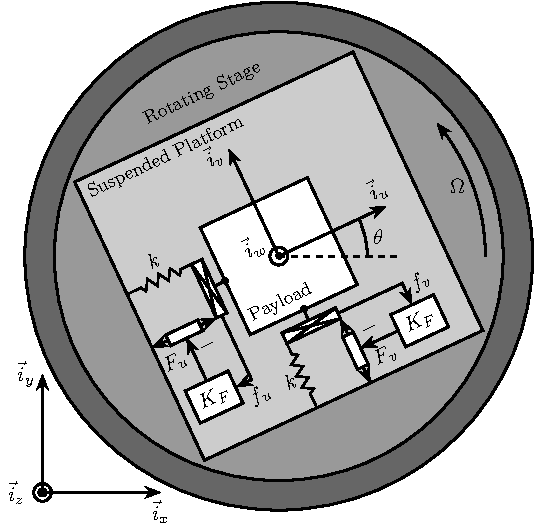
\includegraphics[scale=1]{figs/system_iff.pdf}
\caption{\label{fig:system_iff}System with Force Sensors in Series with the Actuators. Decentralized Integral Force Feedback is used}
\end{figure}

\subsection{Plant Dynamics}
\label{sec:orgf2f22c2}
The forces measured by the force sensors are equal to:
\begin{equation}
\label{eq:measured_force}
  \begin{bmatrix} f_{u} \\ f_{v} \end{bmatrix} =
  \begin{bmatrix} F_u \\ F_v \end{bmatrix} - (c s + k)
  \begin{bmatrix} d_u \\ d_v \end{bmatrix}
\end{equation}

Re-injecting \eqref{eq:tf_d} into \eqref{eq:measured_force} yields:
\begin{equation}
\label{eq:tf_f}
\begin{bmatrix} f_{u} \\ f_{v} \end{bmatrix} = \bm{G}_{f} \begin{bmatrix} F_u \\ F_v \end{bmatrix}
\end{equation}
Where \(\bm{G}_f\) is a \(2 \times 2\) transfer function matrix.

\begin{equation}
\bm{G}_f =
\frac{1}{G_{fp}}
\begin{bmatrix}
  G_{fz} & -G_{fc} \\
  G_{fc} &  G_{fz}
\end{bmatrix}
\end{equation}
with:
\begin{align}
  G_{fp} &= \left( \frac{s^2}{{\omega_0}^2} + 2 \xi \frac{s}{\omega_0} + 1 - \frac{{\Omega}^2}{{\omega_0}^2} \right)^2 + \left( 2 \frac{\Omega}{\omega_0} \frac{s}{\omega_0} \right)^2 \\
  G_{fz} &= \left( \frac{s^2}{{\omega_0}^2} - \frac{\Omega^2}{{\omega_0}^2} \right) \left( \frac{s^2}{{\omega_0}^2} + 2 \xi \frac{s}{\omega_0} + 1 - \frac{{\Omega}^2}{{\omega_0}^2} \right) + \left( 2 \frac{\Omega}{\omega_0} \frac{s}{\omega_0} \right)^2 \\
  G_{fc} &= \left( 2 \xi \frac{s}{\omega_0} + 1 \right) \left( 2 \frac{\Omega}{\omega_0} \frac{s}{\omega_0} \right)
\end{align}

The zeros of the diagonal terms are the roots of \(G_{fz}\) (supposing small damping):
\begin{subequations}
  \begin{align}
    z_1 &= \pm j \omega_0 \sqrt{\frac{1}{2} \sqrt{8 \frac{\Omega^2}{{\omega_0}^2} + 1} + \frac{\Omega^2}{{\omega_0}^2} + \frac{1}{2} } \\
    z_2 &= \pm   \omega_0 \sqrt{\frac{1}{2} \sqrt{8 \frac{\Omega^2}{{\omega_0}^2} + 1} - \frac{\Omega^2}{{\omega_0}^2} - \frac{1}{2} }
  \end{align}
\end{subequations}

The frequency of the two complex conjugate zeros \(z_1\) is between the frequency of the two pairs of complex conjugate poles \(p_1\) and \(p_2\).
This is the expected behavior of a collocated pair of actuator and sensor.

However, the two real zeros \(z_2\) induces an increase of +2 of the slope without change of phase (Figure \ref{fig:plant_iff_compare_rotating_speed}).
This represents non-minimum phase behavior.


The low frequency gain, for \(\Omega < \omega_0\), is no longer zero:
\begin{equation}
\label{low_freq_gain_iff_plan}
  \bm{G}_{f0} = \lim_{\omega \to 0} \left| \bm{G}_f (j\omega) \right| = \begin{bmatrix}
  \frac{- \Omega^2}{{\omega_0}^2 - \Omega^2} & 0 \\
  0  & \frac{- \Omega^2}{{\omega_0}^2 - \Omega^2}
\end{bmatrix}
\end{equation}

It increase with the rotational speed \(\Omega\).

\begin{figure}[htbp]
\centering
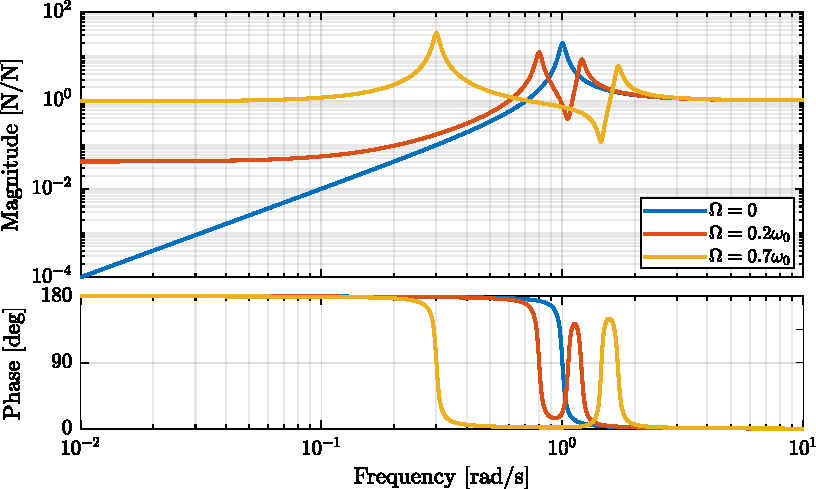
\includegraphics[scale=1]{figs/plant_iff_compare_rotating_speed.pdf}
\caption{\label{fig:plant_iff_compare_rotating_speed}Bode plot of \(\bm{G}_f\) for several rotational speeds \(\Omega\)}
\end{figure}

\subsection{Decentralized Integral Force Feedback}
\label{sec:orge1a14b4}

\begin{equation}
  \bm{K}_F(s) = g \cdot \frac{1}{s}
\end{equation}

Also, as one zero has a positive real part, the \textbf{IFF control is no more unconditionally stable}.
This is due to the fact that the zeros of the plant are the poles of the closed loop system with an infinite gain.
Thus, for some finite IFF gain, one pole will have a positive real part and the system will be unstable.

\begin{figure}[htbp]
\centering
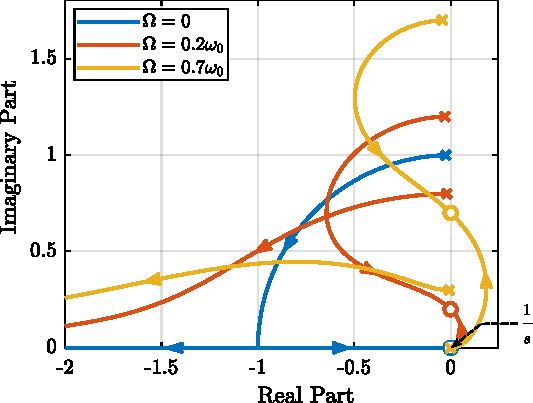
\includegraphics[scale=1]{figs/root_locus_pure_iff.pdf}
\caption{\label{fig:root_locus_pure_iff}Root Locus for the Decentralized Integral Force Feedback}
\end{figure}

At low frequency, the gain is very large and thus no force is transmitted between the payload and the rotating stage.
This means that at low frequency, the system is decoupled (the force sensor removed) and thus the system is unstable.

\section{Integral Force Feedback with High Pass Filters}
\label{sec:org7f551f8}
\subsection{Modification of the Control Low}
\label{sec:org4c39c6d}
\begin{equation}
  \bm{K}_{F}(s) = g \cdot \frac{1}{s} \cdot \underbrace{\frac{s/\omega_i}{1 + s/\omega_i}}_{\text{HPF}} = g \cdot \frac{1}{s + \omega_i}
\end{equation}


\subsection{Feedback Analysis}
\label{sec:org2673698}
\begin{figure}[htbp]
\centering
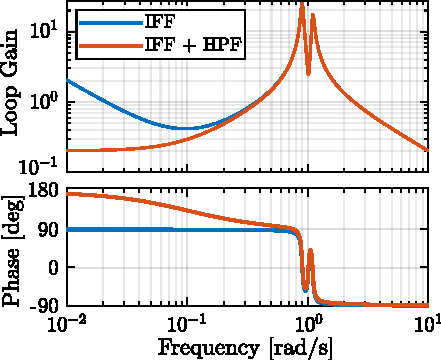
\includegraphics[scale=1]{figs/loop_gain_modified_iff.pdf}
\caption{\label{fig:loop_gain_modified_iff}Bode Plot of the Loop Gain for IFF with and without the HPF}
\end{figure}

\begin{equation}
  g_\text{max} = \omega_i \left( \frac{{\omega_0}^2}{\Omega^2} - 1 \right) \label{eq:iff_gmax}
\end{equation}

\begin{figure}[htbp]
\centering
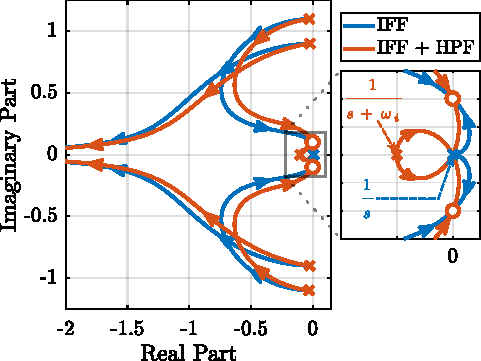
\includegraphics[scale=1]{figs/root_locus_modified_iff.pdf}
\caption{\label{fig:root_locus_modified_iff}Root Locus for IFF with and without the HPF}
\end{figure}

\subsection{Optimal Cut-Off Frequency}
\label{sec:org7d8a789}

\begin{figure}[htbp]
\centering
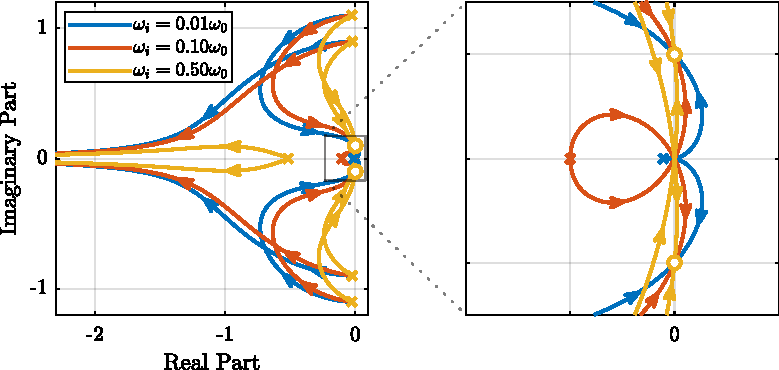
\includegraphics[scale=1]{figs/root_locus_wi_modified_iff.pdf}
\caption{\label{fig:root_locus_wi_modified_iff}Root Locus for several HPF cut-off frequencies \(\omega_i\)}
\end{figure}

\begin{figure}[htbp]
\centering
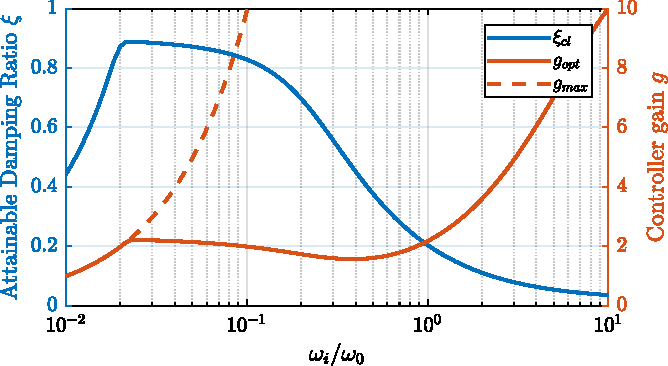
\includegraphics[scale=1]{figs/mod_iff_damping_wi.pdf}
\caption{\label{fig:mod_iff_damping_wi}Attainable damping ratio \(\xi_\text{cl}\) as a function of the HPF cut-off frequency. Corresponding control gain \(g_\text{opt}\) and \(g_\text{max}\) are also shown}
\end{figure}

\section{Integral Force Feedback with Parallel Springs}
\label{sec:org9bc19d0}
\subsection{Stiffness in Parallel with the Force Sensor}
\label{sec:orgdfd59fa}
\begin{figure}[htbp]
\centering
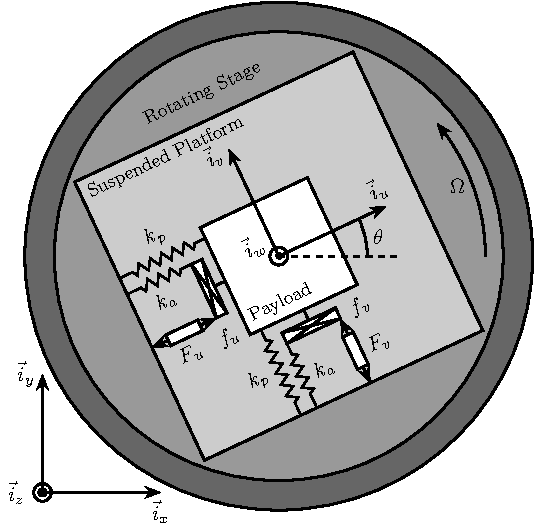
\includegraphics[scale=1]{figs/system_parallel_springs.pdf}
\caption{\label{fig:system_parallel_springs}System with added springs in parallel with the actuators}
\end{figure}

\subsection{Plant Dynamics}
\label{sec:org70fc8fa}

We define an adimensional parameter \(\alpha\), \(0 \le \alpha < 1\), that describes the proportion of the stiffness in parallel with the actuator and force sensor:
\begin{subequations}
  \begin{align}
    k_p &= \alpha k \\
    k_a &= (1 - \alpha) k
  \end{align}
\end{subequations}

The overall stiffness \(k\) stays constant:
\begin{equation}
  k = k_a + k_p
\end{equation}

\begin{equation}
\begin{bmatrix} f_u \\ f_v \end{bmatrix} =
\bm{G}_k
\begin{bmatrix} F_u \\ F_v \end{bmatrix}
\end{equation}

\begin{equation}
\begin{bmatrix} f_u \\ f_v \end{bmatrix} =
\frac{1}{G_{kp}}
\begin{bmatrix}
   G_{kz} & -G_{kc} \\
   G_{kc} &  G_{kz}
\end{bmatrix}
\begin{bmatrix} F_u \\ F_v \end{bmatrix}
\end{equation}
With:
\begin{subequations}
  \begin{align}
    G_{kp} &= \left( \frac{s^2}{{\omega_0}^2} + 2\xi \frac{s}{\omega_0} + 1 - \frac{\Omega^2}{{\omega_0}^2} \right)^2 + \left( 2 \frac{\Omega}{\omega_0}\frac{s}{\omega_0} \right)^2 \\
    G_{kz} &= \left( \frac{s^2}{{\omega_0}^2} - \frac{\Omega^2}{{\omega_0}^2} + \alpha \right) \left( \frac{s^2}{{\omega_0}^2} + 2\xi \frac{s}{\omega_0} + 1 - \frac{\Omega^2}{{\omega_0}^2} \right) + \left( 2 \frac{\Omega}{\omega_0}\frac{s}{\omega_0} \right)^2 \\
    G_{kc} &= \left( 2 \xi \frac{s}{\omega_0} + 1 - \alpha \right) \left( 2 \frac{\Omega}{\omega_0}\frac{s}{\omega_0} \right)
  \end{align}
\end{subequations}

\subsection{Effect of the Parallel Stiffness on the Plant Dynamics}
\label{sec:orge20adc9}
\begin{equation}
  \begin{align}
    \alpha > \frac{\Omega^2}{{\omega_0}^2} \\
    \Leftrightarrow k_p > m \Omega^2
  \end{align}
\end{equation}

\begin{figure}[htbp]
\centering
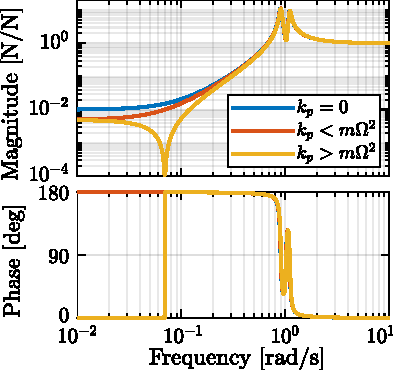
\includegraphics[scale=1]{figs/plant_iff_kp.pdf}
\caption{\label{fig:plant_iff_kp}Bode Plot of \(f_u/F_u\) without parallel spring, with parallel springs with stiffness \(k_p < m \Omega^2\) and \(k_p > m \Omega^2\)}
\end{figure}

\begin{figure}[htbp]
\centering
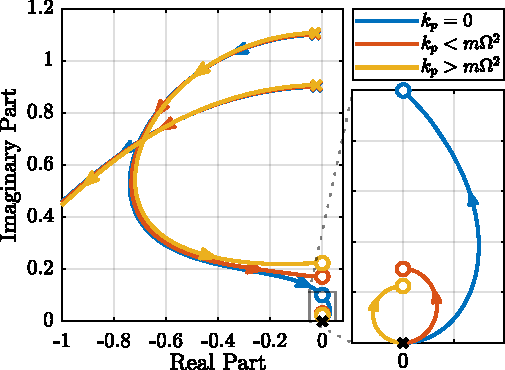
\includegraphics[scale=1]{figs/root_locus_iff_kp.pdf}
\caption{\label{fig:root_locus_iff_kp}Root Locus for IFF without parallel spring, with parallel springs with stiffness \(k_p < m \Omega^2\) and \(k_p > m \Omega^2\)}
\end{figure}

\subsection{Optimal Parallel Stiffness}
\label{sec:orgb14b5c2}
\begin{figure}[htbp]
\begin{subfigure}[c]{0.49\linewidth}
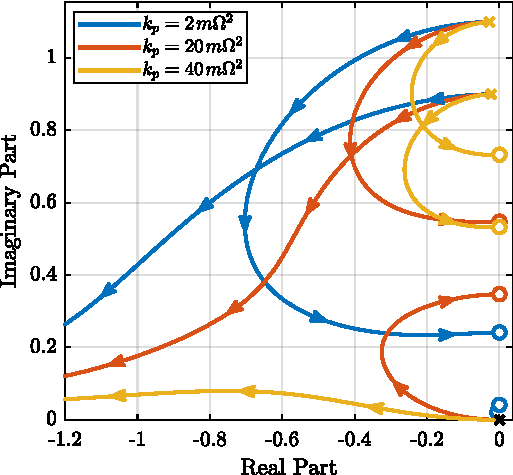
\includegraphics[width=\linewidth]{figs/root_locus_iff_kps.pdf}
\caption{\label{fig:root_locus_iff_kps} Three values of \(k_p\)}
\end{subfigure}
\begin{subfigure}[c]{0.49\linewidth}
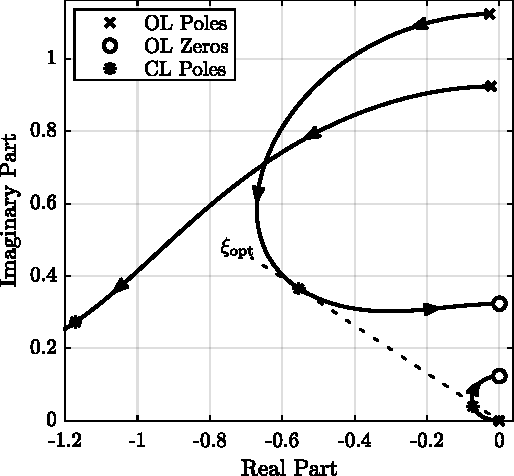
\includegraphics[width=\linewidth]{figs/root_locus_opt_gain_iff_kp.pdf}
\caption{\label{fig:root_locus_opt_gain_iff_kp} \(k_p = 5 m \Omega^2\), optimal damping is shown}
\end{subfigure}
\caption{\label{fig:root_locus_iff_kps_opt}Root Locus for IFF when parallel stiffness is used}
\centering
\end{figure}


\section{Direct Velocity Feedback}
\label{sec:org7628683}
\subsection{System Schematic and Control Architecture}
\label{sec:org6953bc7}
\begin{figure}[htbp]
\centering
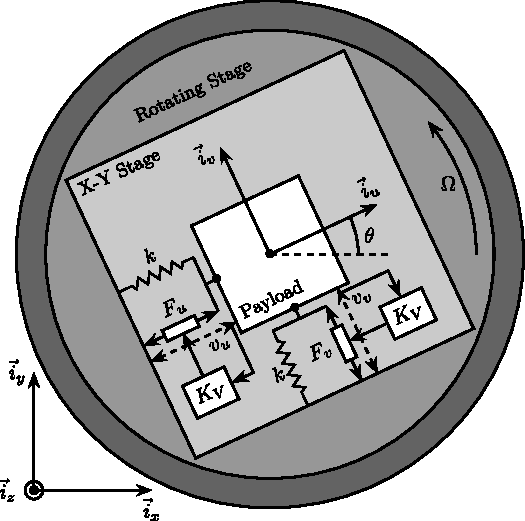
\includegraphics[scale=1]{figs/system_dvf.pdf}
\caption{\label{fig:system_dvf}System with relative velocity sensors and with decentralized controllers \(K_V\)}
\end{figure}

\subsection{Equations}
\label{sec:orgfab42cd}

\begin{equation}
\begin{bmatrix} v_u \\ v_v \end{bmatrix} =
\bm{G}_v
\begin{bmatrix} F_u \\ F_v \end{bmatrix}
\end{equation}

\begin{equation}
\begin{bmatrix} v_u \\ v_v \end{bmatrix} =
\frac{1}{k} \frac{1}{G_{vp}}
\begin{bmatrix}
   G_{vz} & G_{vc} \\
  -G_{vc} & G_{vz}
\end{bmatrix}
\begin{bmatrix} F_u \\ F_v \end{bmatrix}
\end{equation}
With:
\begin{subequations}
  \begin{align}
    G_{vp} &= \left( \frac{s^2}{{\omega_0}^2} + 2 \xi \frac{s}{\omega_0} + 1 - \frac{{\Omega}^2}{{\omega_0}^2} \right)^2 + \left( 2 \frac{\Omega}{\omega_0} \frac{s}{\omega_0} \right)^2 \\
    G_{vz} &= s \left( \frac{s^2}{{\omega_0}^2} + 2 \xi \frac{s}{\omega_0} + 1 - \frac{{\Omega}^2}{{\omega_0}^2} \right) \\
    G_{vc} &= 2 \frac{\Omega}{\omega_0} \frac{s}{\omega_0}
  \end{align}
\end{subequations}


\subsection{Relative Direct Velocity Feedback}
\label{sec:org5cf0d6b}

\begin{figure}[htbp]
\centering
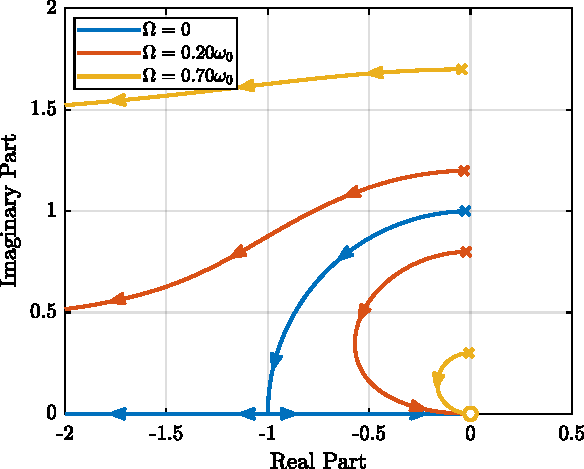
\includegraphics[scale=1]{figs/root_locus_dvf.pdf}
\caption{\label{fig:root_locus_dvf}Root Locus for Decentralized Direct Velocity Feedback for several rotational speeds \(\Omega\)}
\end{figure}

\section{Comparison of the Proposed Active Damping Techniques for Rotating Positioning Stages}
\label{sec:orga2b60a8}
\subsection{Physical Comparison}
\label{sec:orgb69316c}



\subsection{Attainable Damping}
\label{sec:org5c23e13}

\begin{figure}[htbp]
\centering
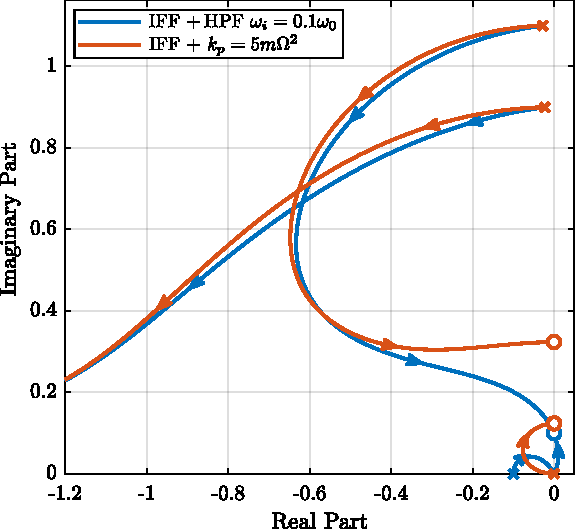
\includegraphics[scale=1]{figs/comp_root_locus.pdf}
\caption{\label{fig:comp_root_locus}Root Locus for the three proposed decentralized active damping techniques: IFF with HFP, IFF with parallel springs, and relative DVF}
\end{figure}


\subsection{Transmissibility and Compliance}
\label{sec:org723fb63}


\begin{figure}[htbp]
\begin{subfigure}[c]{0.45\linewidth}
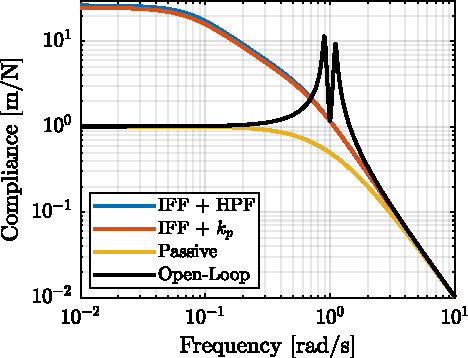
\includegraphics[width=\linewidth]{figs/comp_compliance.pdf}
\caption{\label{fig:comp_compliance} Transmissibility}
\end{subfigure}
\begin{subfigure}[c]{0.45\linewidth}
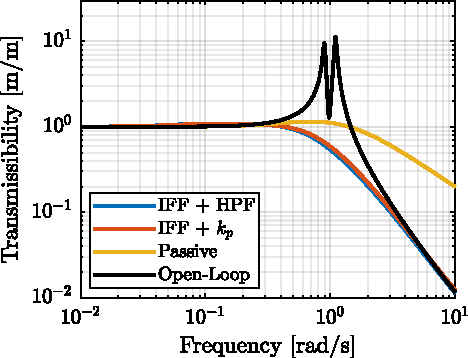
\includegraphics[width=\linewidth]{figs/comp_transmissibility.pdf}
\caption{\label{fig:comp_transmissibility} Compliance}
\end{subfigure}
\caption{\label{fig:comp_active_damping}Comparison of the three proposed Active Damping Techniques}
\centering
\end{figure}

\section{Conclusion}
\label{sec:orgd52b568}
\label{sec:conclusion}

\section*{Acknowledgment}
\label{sec:orge4d73e9}

\bibliography{ref.bib}
\end{document}
